\subsection{Desarrollo de la idea.}

\vspace*{0.3cm}

La heurística de búsqueda local que hemos diseñado, parte de una solución inicial, y a partir de ahí irá encontrando nuevas soluciones ``vecinas''.  Si una solución ``vecina'' resulta ser mejor, es decir, es un conjunto independiente maximal con menos elementos que la solución anterior, entonces la reemplazará.  Estos pasos se repitirán hasta que se encuentre una solución que no pueda mejorarse, es decir, una solución óptima local.

Se analizarán dos posibles soluciones iniciales:

\begin{itemize}
\item La solución hallada por el algoritmo goloso presentado anteriormente.
\item Una solución hallada de la siguiente manera: tomando los nodos del grafo en cierto orden, si el nodo actual no forma parte del conjunto solución ni es adyacente a un nodo del conjunto solución, entonces agregarlo al mismo; en caso contrario, avanzar al siguiente nodo.
\end{itemize}

Para cada solución factible $S$, se define $N(S)$ como el conjunto de ``soluciones vecinas'' de $S$.  Plantearemos dos ``vecindades'' posibles para las soluciones.  

\begin{itemize}
\item {\bf Vecindad 1:} Una solución $S' \in N(S)$ si y sólo si puede obtenerse intercambiando tres nodos de $S$ por dos nodos que no pertenecía a $S$.  Es decir, para $u,v,w \in S$, y $x,y$ nodos del grafo original tal que $x \not \in S$ y $y \not \in S$, definimos $S' = S - \{u,v,w\} + \{x,y\}$ y decimos que $S'$ es ``vecina'' de $S$ si y sólo si $S'$ es un conjunto independiente maximal del grafo original. La Figura \ref{fig:vec1} es un ejemplo de solución ``vecina'' conisderando a la Figura \ref{fig:solinicial} como solución inicial para el grafo de la Figura \ref{fig:estrellita}.  En este caso, se han quitado los nodos 1, 8 y 11 para agregar los nodos 3 y 5.
\item {\bf Vecindad 2:} Una solución $S' \in N(S)$ si y sólo si puede obtenerse agregando a $S$ un nodo del grafo original que no pertenezca a $S$, y quitando todos los nodos de $S$ adyacentes a este nuevo nodo.  Es decir, para $v$ un nodo del grafo original tal que $v \not \in S$, y $A \subseteq S$ tal que para todo $w \in S$, si $w$ es adyacente a $v$ entonces $w \in A$, definimos $S' = S - A + \{v\}$ y decimos que $S'$ es ``vecina'' de $S$ si y sólo si $S'$ es un conjunto independiente maximal del grafo original.  La Figura \ref{fig:vec2} es un ejemplo de solución ``vecina'' conisderando a la Figura \ref{fig:solinicial} como solución inicial para el grafo de la Figura \ref{fig:estrellita}.  En este caso, se ha agregado el nodo 2 y se han quitado los nodos 1, 6 y 7.
\end{itemize}

 
\begin{figure}[!htb]
\minipage{0.5\textwidth}
\begin{center}
  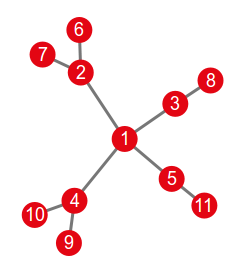
\includegraphics[scale=0.8]{imagenes/estrellita.png}
\end{center}
  \caption{Ejemplo de grafo}\label{fig:estrellita}
\endminipage\hfill
\minipage{0.5\textwidth}
\begin{center}
  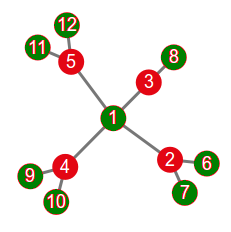
\includegraphics[scale=0.8]{imagenes/estrellitasolinicial.png}
\end{center}
  \caption{Posible solución inicial}\label{fig:solinicial}
\endminipage
\vspace*{0.3cm}
\minipage{0.5\textwidth}%
\begin{center}
  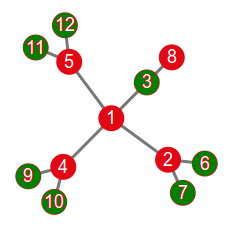
\includegraphics[scale=0.8]{imagenes/estrellitavec1.png}
\end{center}
  \caption{Solución vecina según Vecindad 1}\label{fig:vec1}
\endminipage\hfill
\minipage{0.5\textwidth}
\begin{center}
  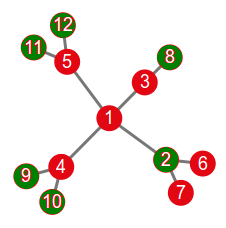
\includegraphics[scale=0.8]{imagenes/estrellitavec2.png}
\end{center}
  \caption{Solución vecina según Vecindad 2}\label{fig:vec2}
\endminipage
\end{figure}
 
 
\vspace*{0.6cm}

%\newpage

\subsection{Análisis de complejidad de una iteración.}

Para analizar la complejidad del algoritmo en este caso, tendremos que hacer una división en dos casos, con mejorador1 y con mejorador2.
Debemos señalar que conseguir la solución inicial no formará parte del análisis de complejidad dado que es un factor externo, por no estar incluido dentro de una iteración del algoritmo.

En el caso de hacer uso de mejorador1, el procedimiento a realizar en una iteración consiste en obtener un grupo de 3 nodos (esto se hace con 3 iteraciones distintas sobre los elementos de la solución, siendo $\mathcal{O}(n)$ cada iteración y llegando a un costo posible de $\mathcal{O}(n^3)$). Por cada posible combinación de estos 3 nodos, se modifican ciertas variables internas para simular la eliminación de estos elementos (toma $3\mathcal{O}(n)$ ya que implica recorrer los vecinos de estos 3 nodos) y se buscan 2 candidatos entre sus vecinos (uniendo los conjuntos de vecinos de los 3 nodos y eliminando los repetidos), mediante 2 iteraciones anidadas sobre el conjunto de vecinos y verificando si resultan viables ($\mathcal{O}(1)$ la verificación y $\mathcal{O}(n^2)$ encontrar los 2 candidatos, en caso de que los haya). En caso de que se cumplan las condiciones para modificar la solución actual, termina la iteración, de lo contrario, se deshacen las modificaciones realizadas ($3\mathcal{O}(n)$) y termina la iteración.

Con esta información, y siendo $T(n)$ la complejidad de nuestro algoritmo, tenemos:

\begin{equation*}
\begin{array}{l}
T(n) = \mathcal{O}(n^3) * \mathcal{O}(n^2) + 3\mathcal{O}(n) + 3\mathcal{O}(n) \\
T(n) = \mathcal{O}(n^5) + 6\mathcal{O}(n) \\
T(n) = \mathcal{O}(n^5)
\end{array}
\end{equation*}

En el caso de utilizar mejorador2, el procedimiento es distinto. Partimos buscando nodos que se relacionen con al menos dos nodos de la solución inicial (preguntar por cada nodo nos toma $\mathcal{O}(n)$). Por cada nodo que cumpla, se actualizan variables relacionadas con ese nodo para simular su incorporación a la solución (para esto se requiere recorrer los vecinos de ese nodo con costo $\mathcal{O}(n)$). Luego revisamos si incorporando el nodo previamente seleccionado llegamos a una solución válida ($\mathcal{O}(n)$), de ser así, quitamos los nodos que se relacionan con éste, modificamos variables para seguir teniendo en cuenta el cambio realizado ($\mathcal{O}(n)$) y terminamos la iteración. En caso contrario, terminamos la iteración (al no modificar las variables del otro caso, estas se verán reseteadas en la siguiente iteración).

En este caso, siendo $T(n)$ la complejidad de nuestro algoritmo, tenemos:

\begin{equation*}
\begin{array}{l}
T(n) = \mathcal{O}(n) * \mathcal{O}(n) + \mathcal{O}(n) + \mathcal{O}(n)\\
T(n) = \mathcal{O}(n^2) + 2\mathcal{O}(n) \\
T(n) = \mathcal{O}(n^2)
\end{array}
\end{equation*}

\vspace*{0.3cm}

\begin{figure}
\begin{codebox}
\Procname{$\proc{CIDM_busqueda}(int$ $mej)$}
\li $cidm\_sol \leftarrow$ lista de nodos de una solución inicial
\li $res \leftarrow |cidm\_sol|$
\li \While haya mejoras y la última solución tenga más de un nodo
\li \Do 
		\If $mej == 1$
\li 		\Then {\sc mejorador1}($cidm\_sol,res$)
\li 		\Else {\sc mejorador2}($cidm\_sol,res$)
		\End
	\End
\end{codebox}
\caption{Heurística de búsqueda local para CIDM}\label{code:busqueda}
\end{figure}
%\FloatBarrier


\begin{figure}
\begin{codebox}
\Procname{$\proc{Mejorador1}(lista\_nodos$ $cidm\_sol,int$ $res)$} 
\li \For cada grupo de 3 de nodos en $cidm\_sol$
\li \Do 
		``sacar'' los 3 nodos
\li 		\For cada par de vecinos $n1,n2$ de estos nodos
\li 		\Do 
			\If $n1$ y $n2$ quedaron ``libres'' y no son adyacentes
\li			\Then
				``agregar'' $n1$ y $n2$
\li 				\If se forma una solución válida
\li 				\Then salir del ciclo
				\End
			\End
		\End
\li 		\If se encontró una solución mejor
\li 		\Then
			actualizar $cidm\_sol$
\li 			actualizar $res$
\li 			\Return
		\End
	\End
\li \Return
\end{codebox}
\caption{Pseudocódigo de la mejora 1}\label{code:mej1}
\end{figure}
%\FloatBarrier



\begin{figure}
\begin{codebox}
\Procname{$\proc{Mejorador2}(lista\_nodos$ $cidm\_sol,int$ $res)$} 
\li \For cada nodo $n$
\li \Do 
		\If $n$ se conecta con al menos dos nodos de $cidm\_sol$
\li 		\Then 
			\For cada nodo de $cidm\_sol$ que se conecta a $n$
\li 			\Do 
				``sacar'' el nodo
\li 				\If se forma una solución válida
\li 				\Then salir del ciclo
				\End
			\End
\li 			\If se encontró una solución mejor
\li 			\Then
				actualizar $cidm\_sol$
\li 				actualizar $res$
\li 				\Return
			\End
		\End
	\End
\li \Return
\end{codebox}
\caption{Pseudocódigo de la mejora 2}\label{code:mej2}
\end{figure}
%\FloatBarrier


\vspace*{0.6cm}
\newpage
\subsection{Experimentación y gráficos.}

\vspace*{0.3cm}

En esta sección trataremos de encontrar, entre las posibles combinaciones de soluciones iniciales y vecindades explicadas anteriormente, aquella que tenga el mejor balance entre calidad de solución y performance. 

Para facilitar la lectura, nombraremos a cada configuracón de la siguiente manera:

\begin{itemize}
	\item {\bf Configuración 1:} Utiliza como solución inicial la hallada por nuestra heurística golosa, y busca mejorar la solución con la Vecindad 1.
	\item {\bf Configuración 2:} Utiliza como solución inicial la hallada por el algoritmo no goloso, y busca mejorar la solución con la Vecindad 1.
	\item {\bf Configuración 3:} Utiliza como solución inicial la hallada por nuestra heurística golosa, y busca mejorar la solución con la Vecindad 2.
	\item {\bf Configuración 4:} Utiliza como solución inicial la hallada por el algoritmo no goloso, y busca mejorar la solución con la Vecindad 2.

\end{itemize}

Plantearemos entonces, experimentos que nos permitan observar cómo se desenvuelve nuestro algoritmo con cada configuración, y con los resultados, tratar de elegir una de ellas. Para ello se ha decidido evaluar instancias de tipo $circuito$, $estrella$, $galaxia$ y $aleatorio$.
 
\subsubsection{Circuitos}

Se generaron 45 $circuitos$ con entre 5 y 50 nodos.  El orden de los nodos fue aleatorizado para no depender de un rotulado en particular.

\paragraph{Performance} 

El gráfico obtenido con las mediciones de tiempo es el que se muestra en la Figura \ref{fig:3A}.

\begin{figure}[htb]
	\begin{center}
    		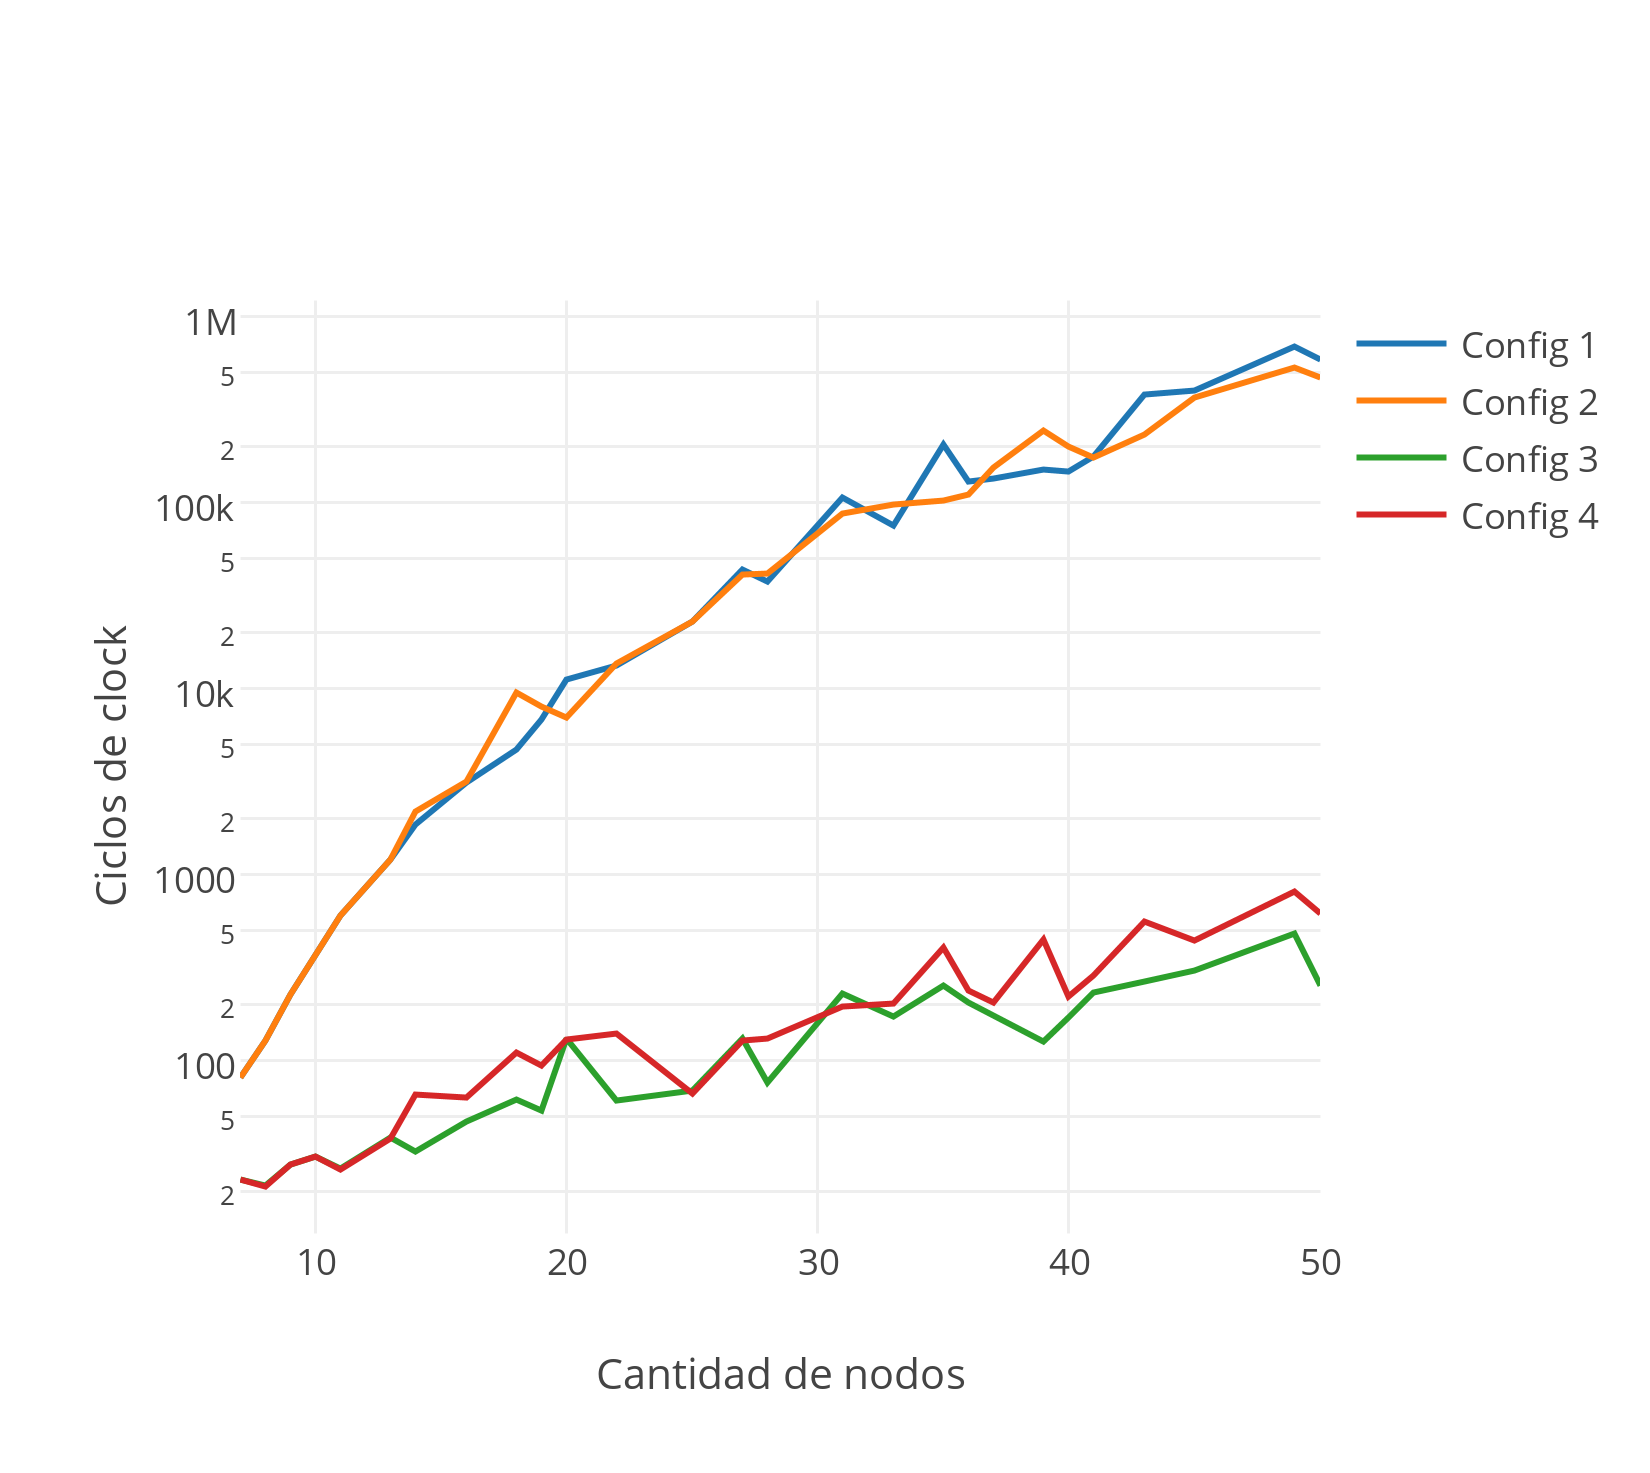
\includegraphics[scale=0.8]{imagenes/busqlocal-circuitos-tiempo.png}
	\end{center}
	\caption{Búsqueda local - Circuitos}\label{fig:3A}
\end{figure}
%\FloatBarrier

La Figura parece indicar que aquellas configuraciones que utilizan la Vecindad 1  tienen un desempeño peor que aquellas que utilizan la Vecindad 2, y en la medida que se incrementa la cantidad de nodos la diferencia se hace más evidente. Además, entre las configuraciones que utilizan la Vecindad 2, la número 3 es la que aparenta tener un mejor rendimiento sobre las instancias evaluadas.

\paragraph{Calidad} Se ha comparado el tamaño de la solución hallada con el tamaño de la solución exacta.  Los porcentajes de desaciertos sobre el total de instancias evaluadas son los siguientes:

\begin{verbatim}
Configuración 1: 34%
Configuración 2: 32%
Configuración 3: 54%
Configuración 4: 54%
\end{verbatim}

En este caso, el menor porcentaje de error fue logrado por aquellas configuraciones que utilizan a la Vecindad 1.  De todos modos, se trata de un porcentaje bastante alto.

\subsubsection{Estrellas}

Se generaron 60 grafos $estrellas$ con grado máximo entre 5 y 10.

\paragraph{Performance}

La Figura \ref{fig:3B} muestra los resultados obtenidos respecto al tiempo de ejecución. Nuevamente, las configuraciones que utilizan la Vecindad 2 muestran un desempeño considerablemente mejor en términos de performance que aquellas que utilizan la Vecindad 1.

\begin{figure}[htb]
	\begin{center}
    		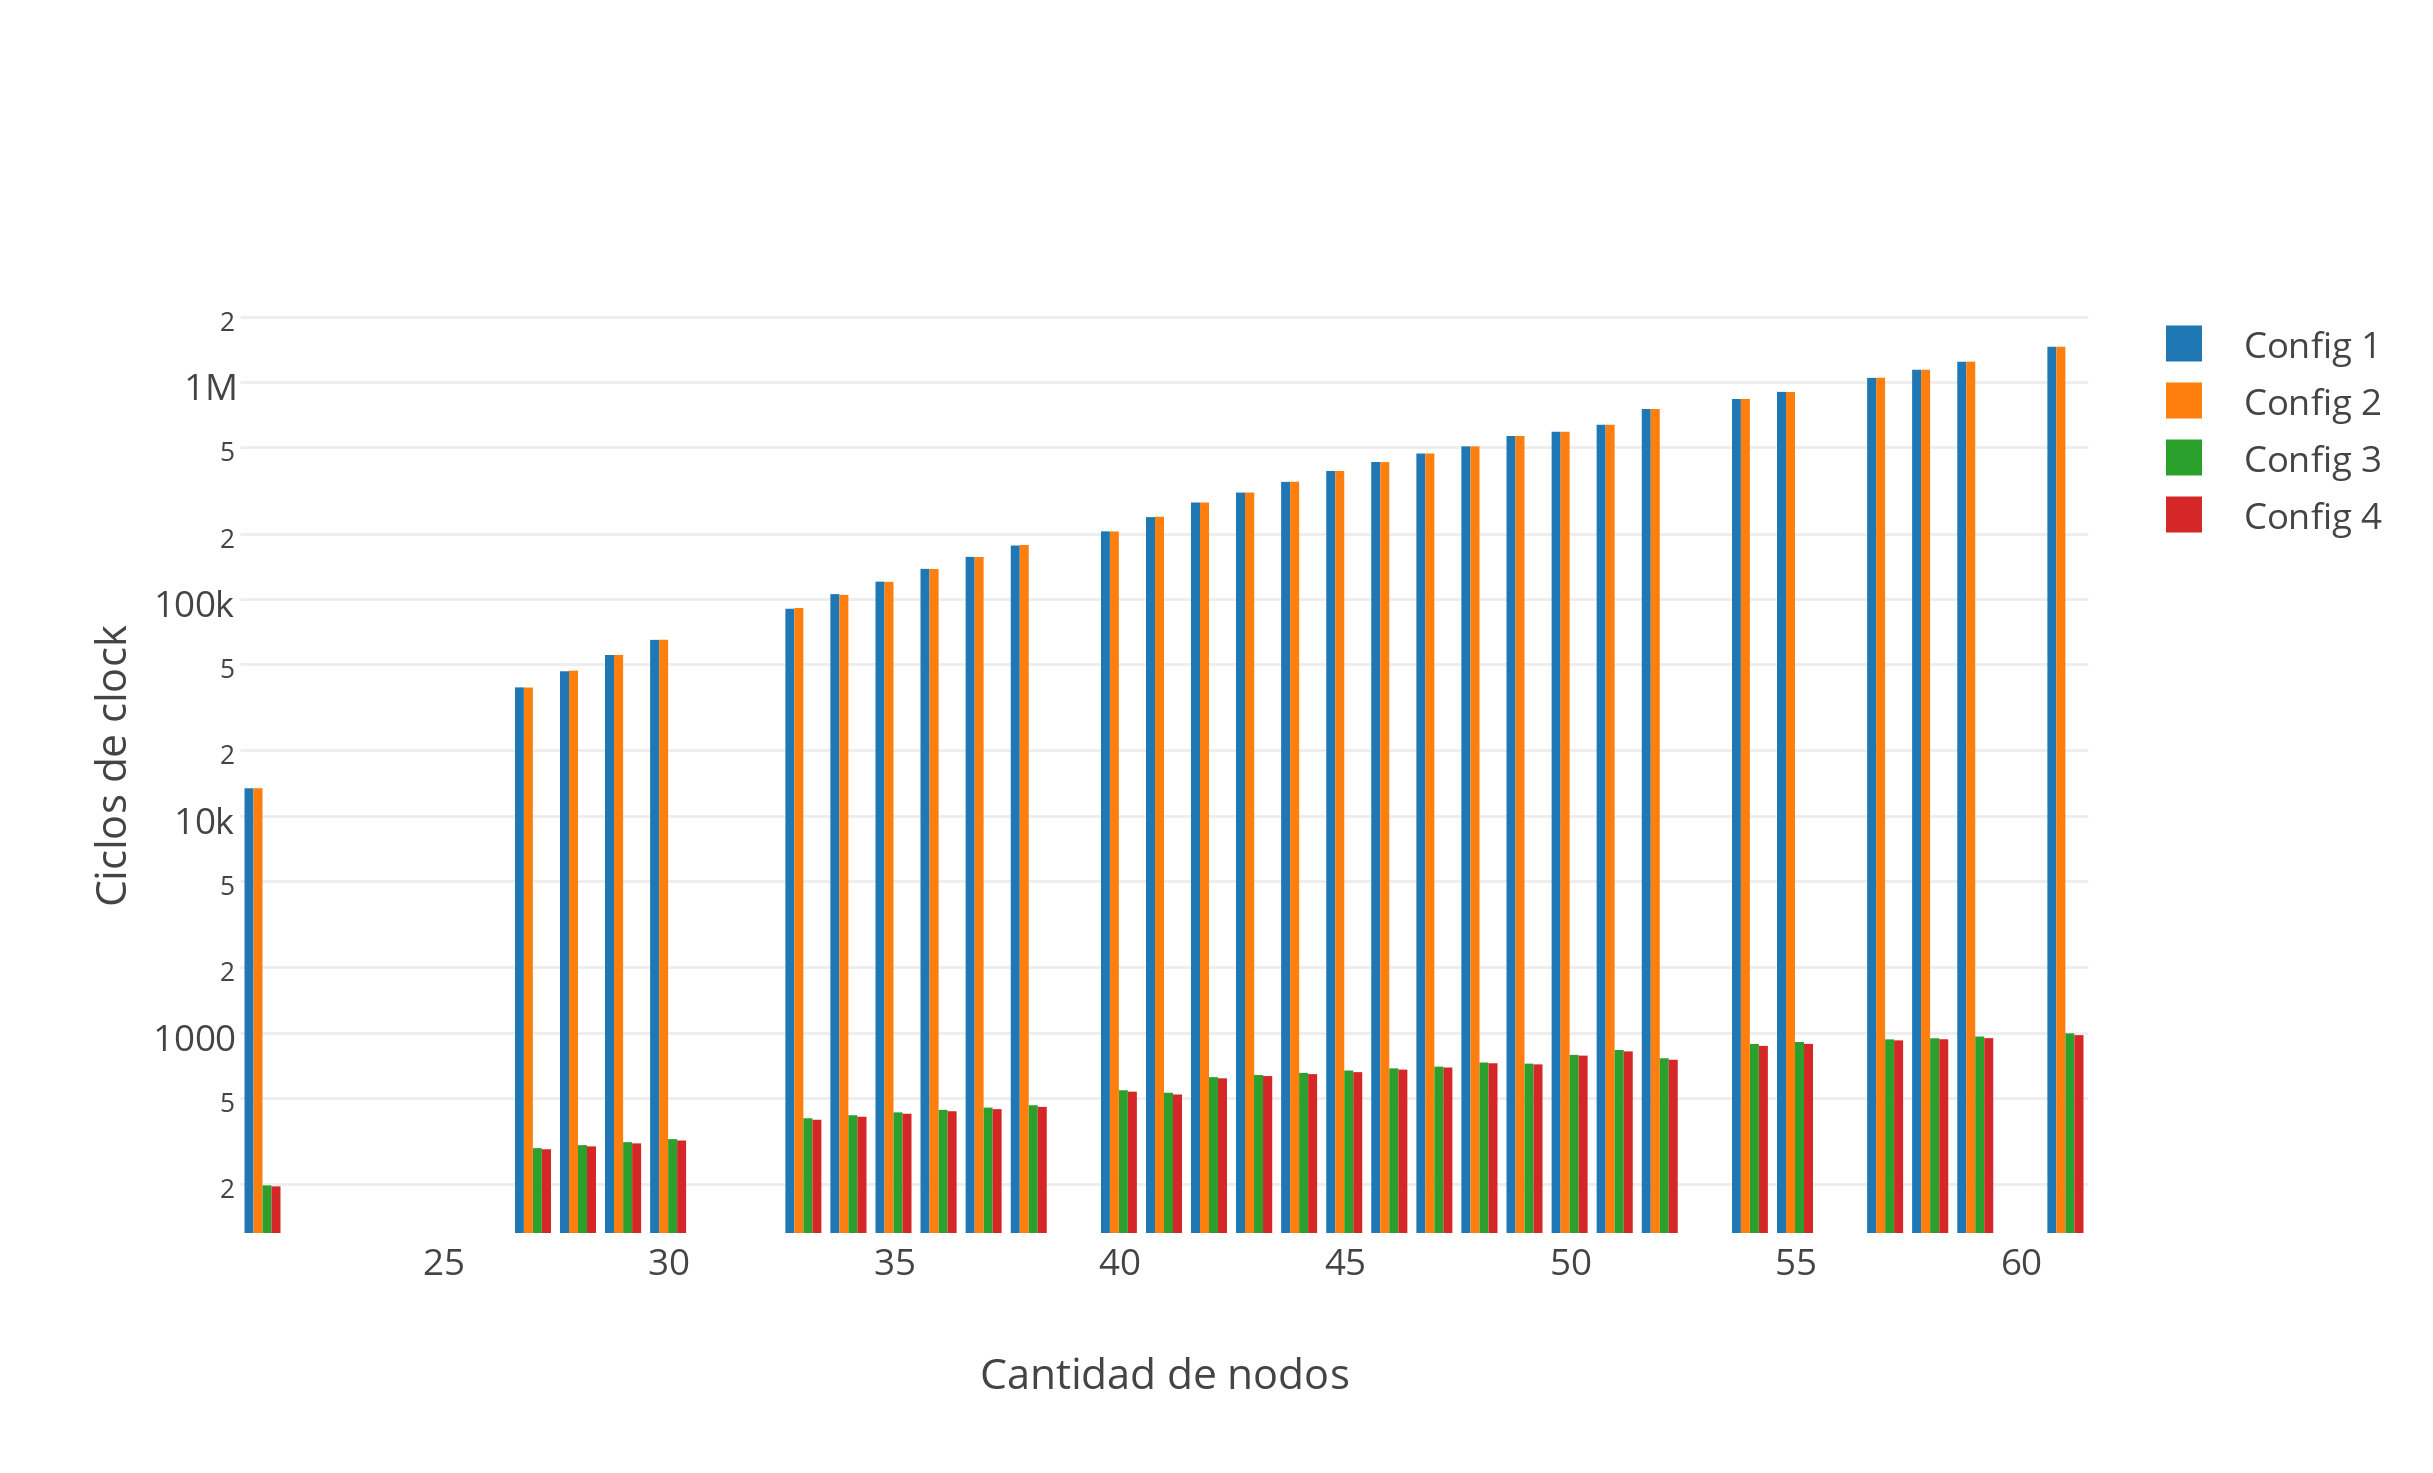
\includegraphics[scale=0.8]{imagenes/busqlocal-estrellas-tiempo.png}
	\end{center}
	\caption{Búsqueda local - Estrellas}\label{fig:3B}
\end{figure}
%\FloatBarrier

\paragraph{Calidad} Para estas instancias, ambas soluciones iniciales se encontraron lejos de la solución exacta. Así que se ha comparado el tamaño de la solución mejorada con el tamaño de la solución exacta, y la calidad de las mejoras obtenidas.  Los porcentajes de desaciertos sobre el total de instancias evaluadas son los siguientes:

\begin{verbatim}
Configuración 1: 100%
Configuración 2: 100%
Configuración 3: 0%
Configuración 4: 0%
\end{verbatim}

Las configuraciones que utilizan la Vecindad 1 no sólo no tuvieron ningún acierto sino que además no mostraron mejora alguna respecto de las soluciones iniciales, mientras que las configuraciones que utilizan la Vecindad 2 lograron mejorar completamente ambas soluciones iniciales.

\subsubsection{Galaxias}

Se generaron 40 grafos $galaxia$ con entre 35 y 115 nodos.

\paragraph{Performance}

La Figura \ref{fig:3C} muestra los resultados obtenidos respecto al tiempo de ejecución. Nuevamente, las configuraciones que utilizan la Vecindad 2 muestran un desempeño considerablemente mejor en términos de performance que aquellas que utilizan la Vecnidad 1, y entre las configuraciones que utilizan la Vecindad 2, la configuración 3 se muestra claramente como la más óptima.

\begin{figure}[htb]
	\begin{center}
    		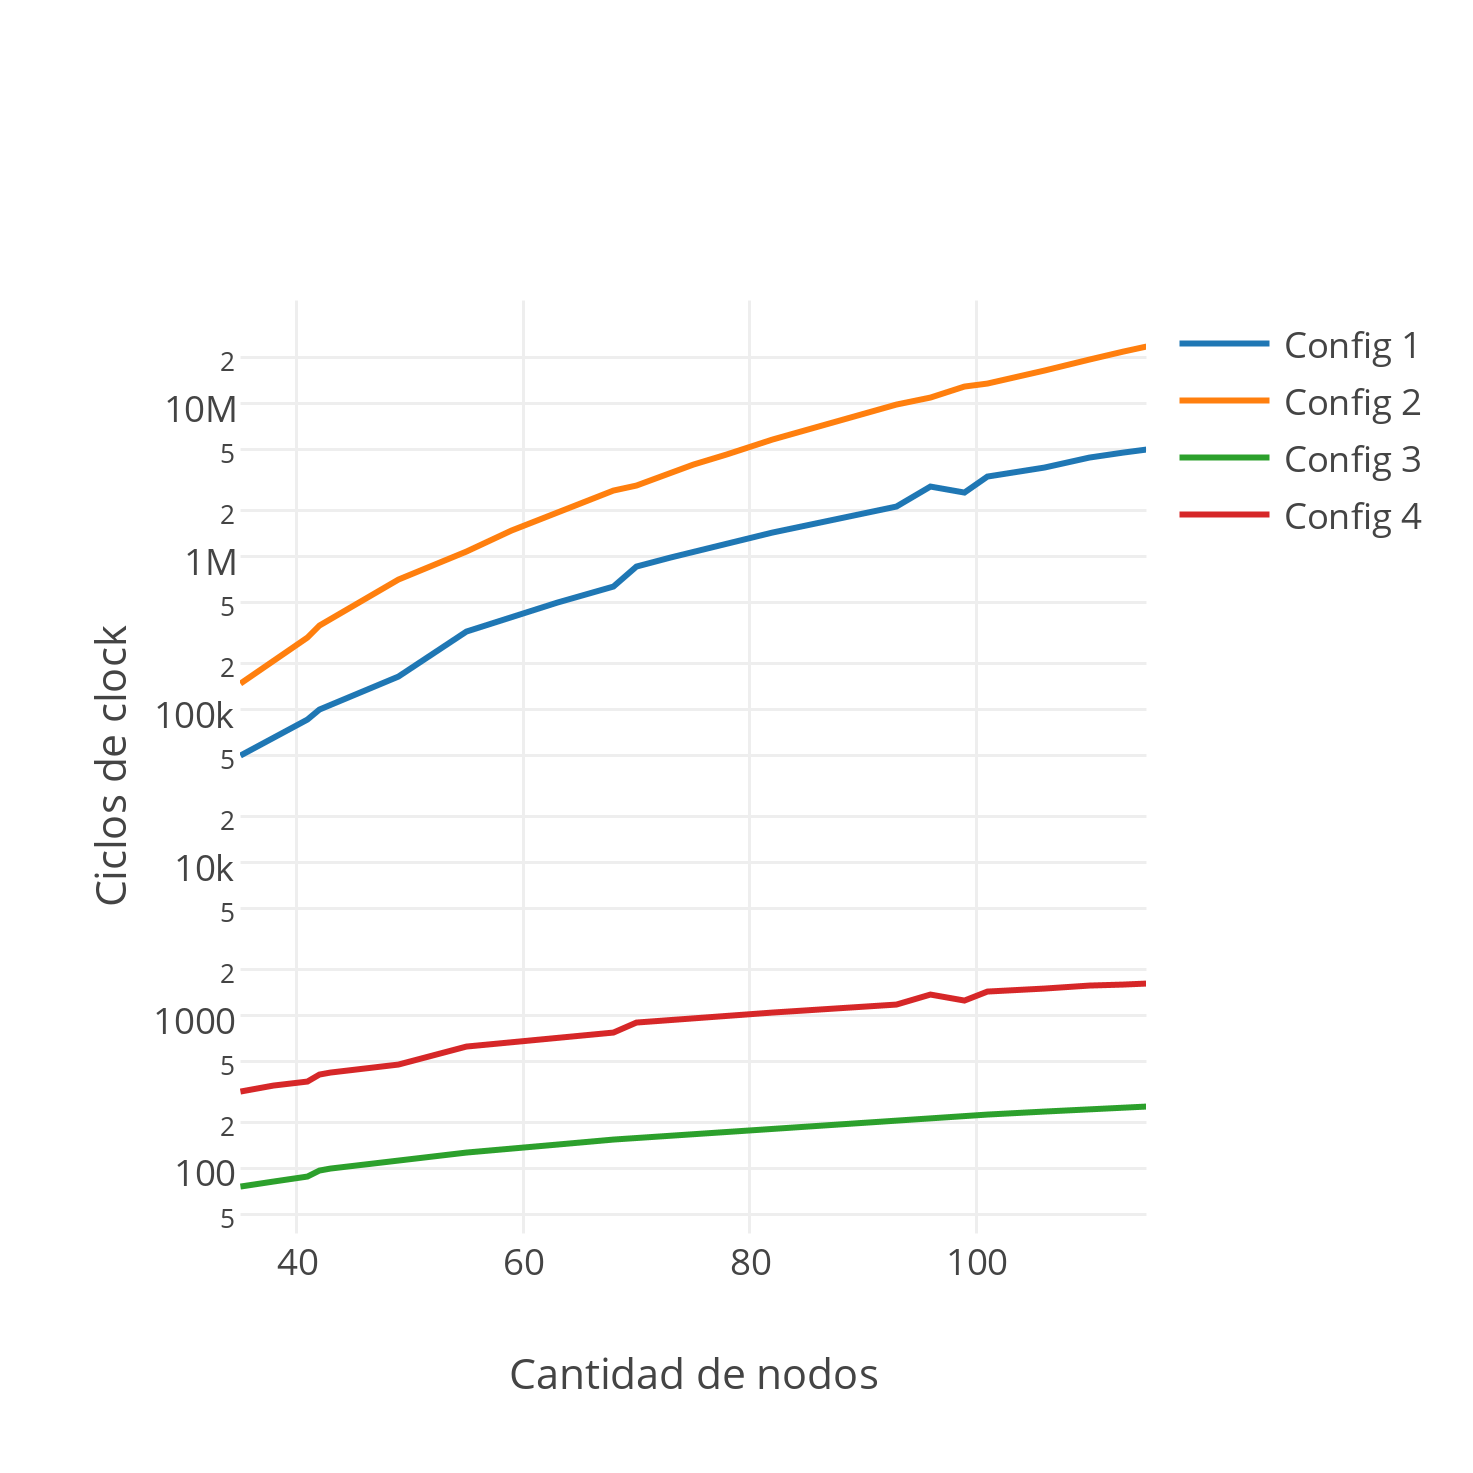
\includegraphics[scale=0.8]{imagenes/busqlocal-galaxias-tiempo.png}
	\end{center}
	\caption{Búsqueda local - Galaxias}\label{fig:3C}
\end{figure}
%\FloatBarrier

\paragraph{Calidad} Para estas instancias, la solución inicial provista por nuestra heurística golosa fue la exacta, mientras que la solución inicial alternativa se encontró lejos de la solución exacta. Así que se ha comparado el tamaño de la solución mejorada con el tamaño de la solución exacta, y la calidad de las mejoras obtenidas.  Los porcentajes de desaciertos sobre el total de instancias evaluadas son los siguientes:

\begin{verbatim}
Configuración 1: 0%
Configuración 2: 100%
Configuración 3: 0%
Configuración 4: 0%
\end{verbatim}

La Configuración 2 no sólo no tuvo ningún acierto sino que además no mostró mejora alguna respecto de la solución inicial, mientras que la Configuración 4 logró mejorarla completamente.  Es importante destacar que, dado que las Configuraciones 1 y 3 partieron de una solución inicial exacta, no aportan información significativa respecto de las mejoras.

\subsubsection{Aleatorios}

Para estos experimentos se han generado dos sets de instancias $aleatorias$. Uno contiene 120 grafos de entre 4 y 15 nodos, para poder contrastar con el algoritmo exacto (sólo se utilizara para la parte de calidad). El otro contiene 460 grafos de entre 4 y 50 nodos, que si bien no serán comparadas con el algoritmo exacto, posibilitará apreciar los tiempos de ejecución más ampliamente y tener una idea más general respecto a la calidad de las soluciones obtenidas.

\paragraph{Performance} La Figura \ref{fig:3D} muestra los resultados obtenidos respecto al tiempo de ejecución. Podemos apreciar que las configuraciones que utilizan la Vecnidad 1 tienen, en general, un desempeño peor que las otras, y entre las configuraciones que utilizan la Vecindad 2, la configuración 3 parecería mostrarse como la más óptima.

\begin{figure}[htb]
	\begin{center}
    		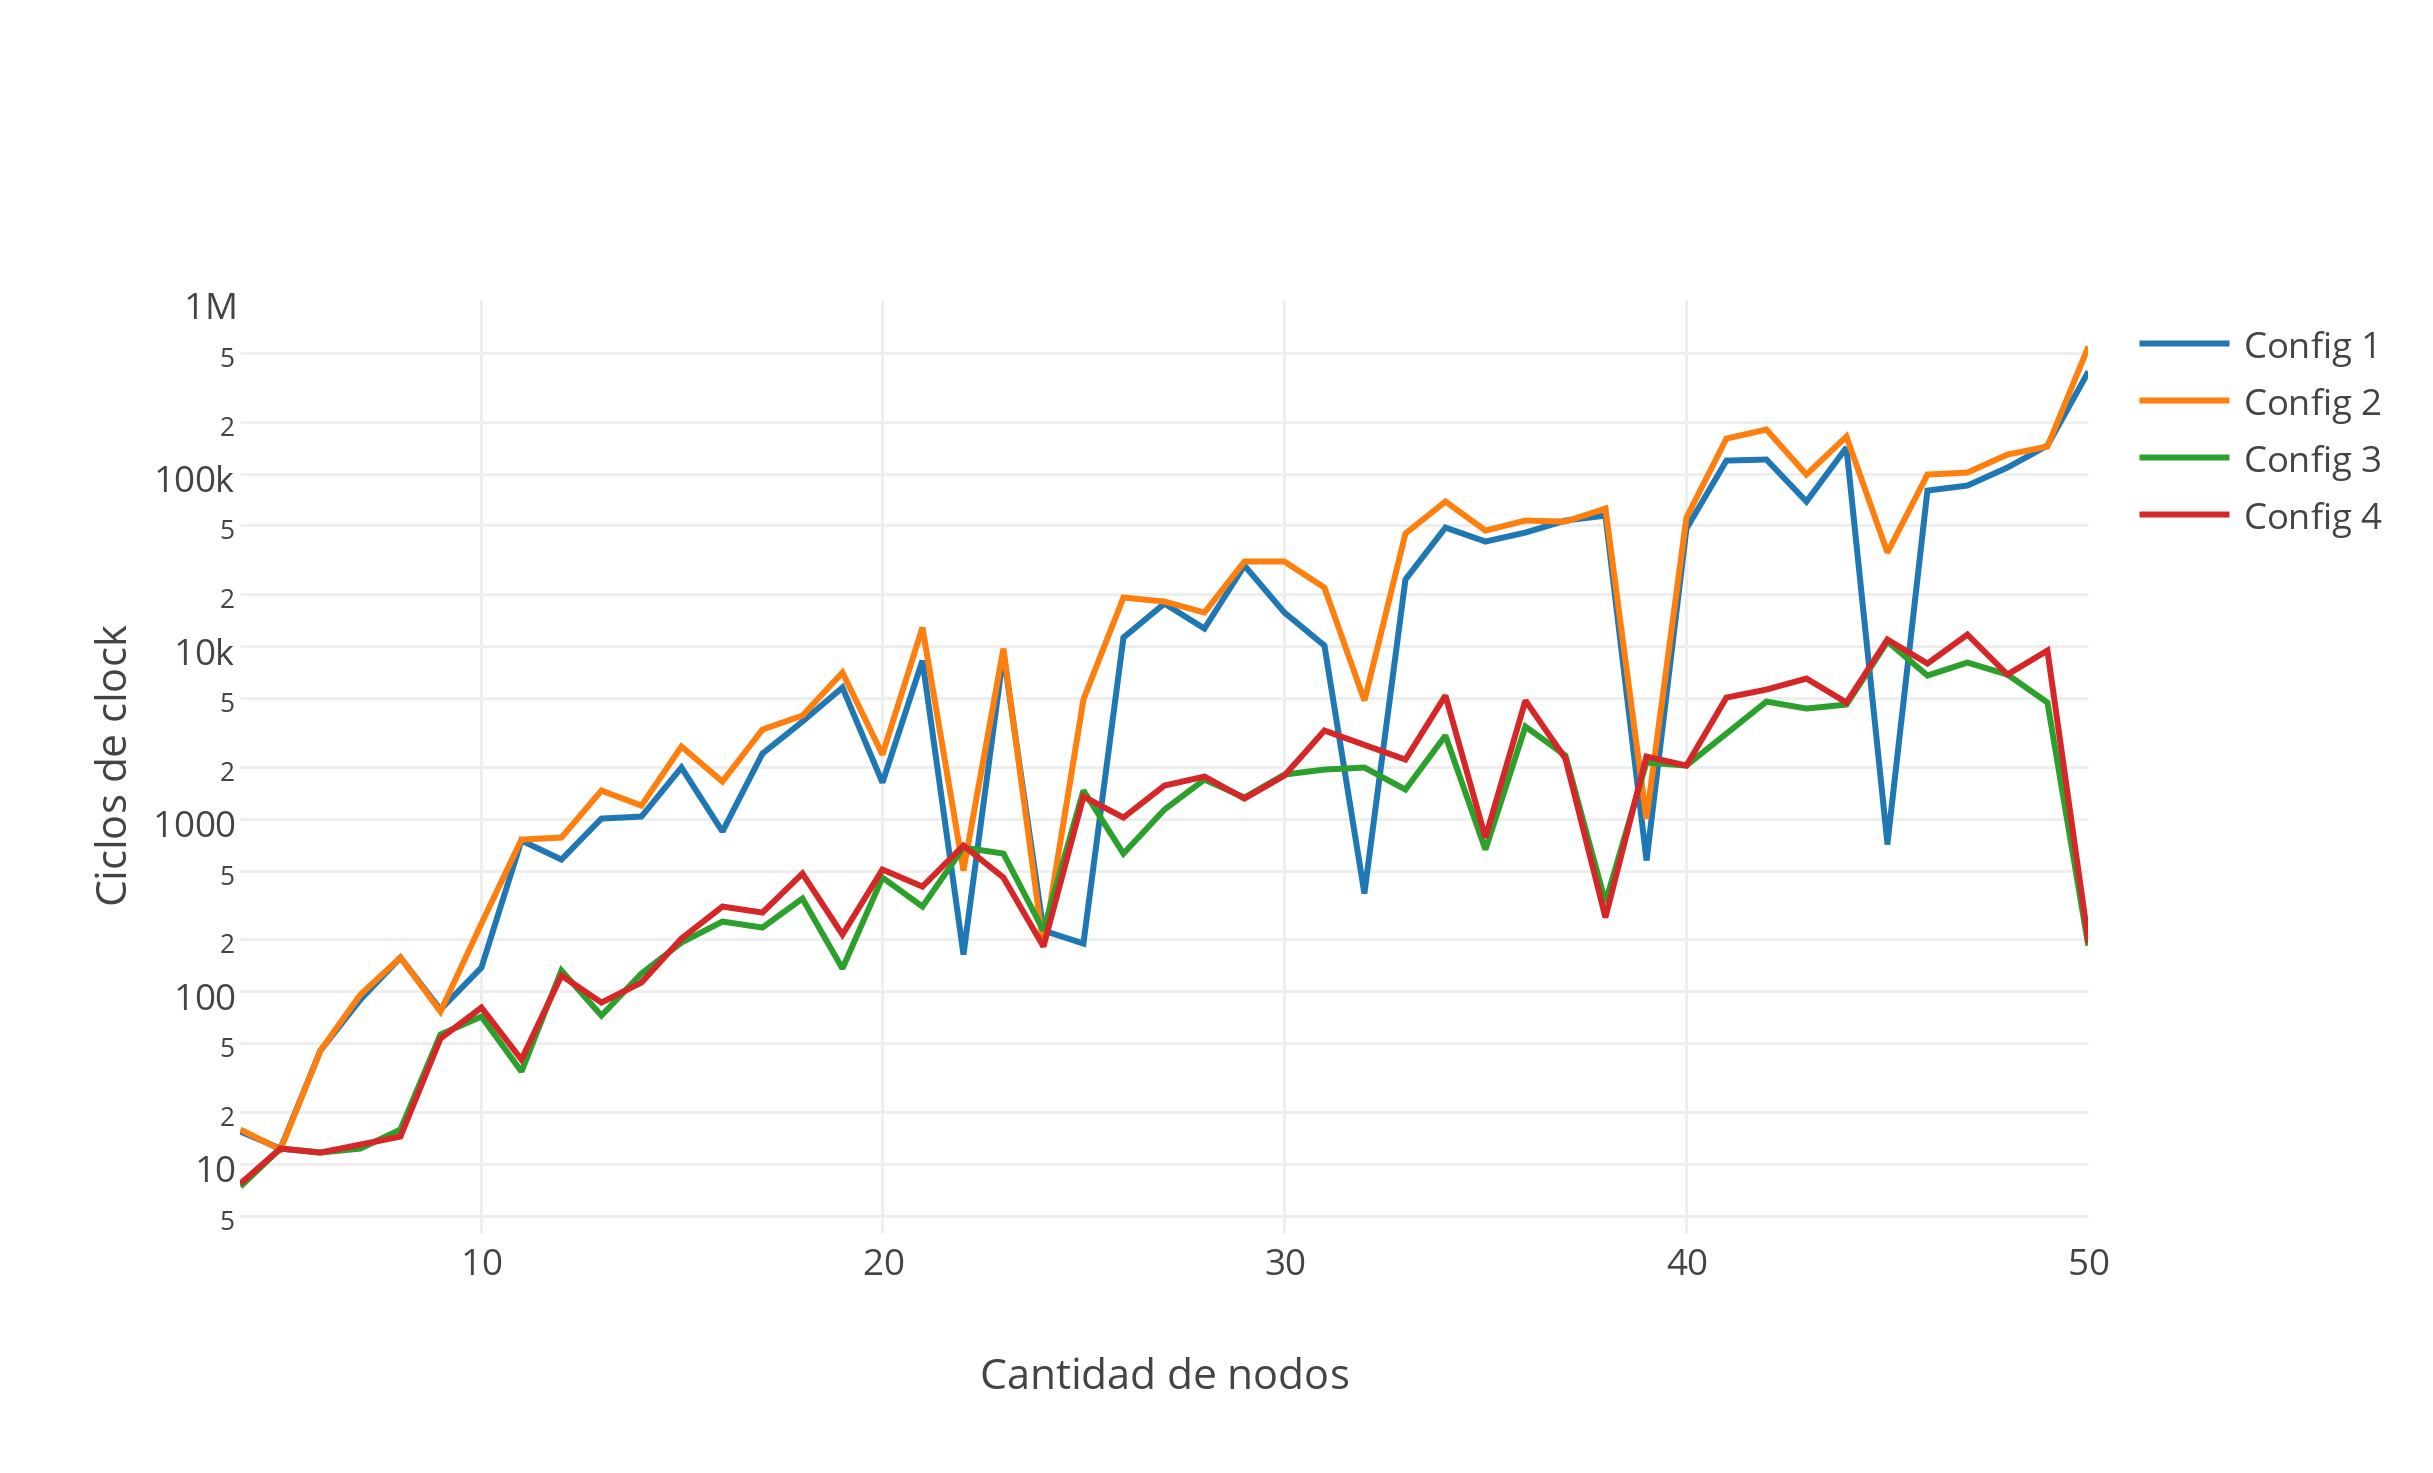
\includegraphics[scale=0.8]{imagenes/busqlocal-aleatorios-tiempo.png}
	\end{center}
	\caption{Búsqueda local - Aleatorios}\label{fig:3D}
\end{figure}
%\FloatBarrier

\paragraph{Calidad} 

\subparagraph{Set 1} Se ha comparado el tamaño de la solución obtenida con el tamaño de la solución exacta.  Los porcentajes de desaciertos sobre el total de instancias evaluadas son los siguientes:

\begin{verbatim}
Configuración 1: 0.833%
Configuración 2: 38.333%
Configuración 3: 2.5%
Configuración 4: 7.5%
\end{verbatim}

La Configuración 2 muestra un porcentaje de desaciertos muy elevado respecto de las demás, mientras que la Configuración 1 se presenta como la más acertada.  Sin embargo, el porcentaje de error de la Configuración 3 no se aleja tanto de la Configuración 1.

\subparagraph{Set 2} Como por el tamaño de estas instancias se dificulta la comparación con el algoritmo exacto, se consideró como la solución ``óptima'' en cada caso el menor valor obtenido entre las cuatro configuraciones, y se registró, para cada una, la cantidad de instancias en las que no se logró dicho valor. Los porcentajes de estos ``desaciertos'' sobre el total de instancias evaluadas son los siguientes:

\begin{verbatim}
Configuración 1: 4.68%
Configuración 2: 26.59%
Configuración 3: 9.57%
Configuración 4: 21.7%
\end{verbatim}

Contrastando con los porcentajes obtenidos para el Set 1 de instancias, la Configuración 2 sigue siendo la que arroja peores resultados, aunque esta vez en un porcentaje menor, mientras que las demás incrementaron su porcentaje de error.  De todos modos, la Configuración 1 vuelve a ser la que obtiene mejores resultados, seguido de cerca por la Configuración 3, y la Configuración 4 se muestra con un margen de error más cercano a la peor.

\subsubsection{Conclusiones} 

Luego de realizar este análisis para distintas instancias, podemos observar que, en lo que respecta a la calidad de las soluciones obtenidas, las configuraciones 1 y 3 muestran, en general logran obtener mejores resultados, con un margen de error similar. Por otro lado, las configuraciones que utilizan la Vecindad 1 requieren un tiempo de ejecución considerablemente mayor que aquellas que utilizan la Vecindad 2.  Por este motivo, si bien la Configuración 1 es la que se muestra mejor en calidad, decidimos considerar a la Configuración 3 como la que mejor balancea calidad y performance.